\documentclass[a4paper, 11pt]{article}
\usepackage[a4paper, left=3cm, bottom=4cm, right=3cm]{geometry}

\RequirePackage[english]{babel}
\RequirePackage[utf8]{inputenc}
\RequirePackage{amsmath}
\RequirePackage{amsfonts}
\usepackage{mathtools}
\RequirePackage{hyperref}
\usepackage{tikz}
\usepackage{braket}

\newcommand{\dd}{\mathop{\mathrm{d}\!}{}}
\newcommand{\Tr}{\mathop{\mathrm{Tr}\!}{}}
\newcommand{\deriv}[2]{\dfrac{\dd #1}{\dd #2}}
\newcommand{\pderiv}[2]{\dfrac{\partial #1}{\partial #2}}
\newcommand{\HH}{\mathcal{H}}

\newcommand\braa[1]{{\langle\langle{#1}|}}
\newcommand\kett[1]{{|{#1}\rangle\rangle}}

\renewcommand\bra[1]{{\langle{#1}|}}
\makeatletter
\renewcommand\ket[1]{%
	\@ifnextchar\bra{\k@t{#1}\!}{\k@t{#1}}%
}
\newcommand\k@t[1]{{|{#1}\rangle}}
\makeatother

\bibliographystyle{alpha}

\date{\today}
\author{Bruno Bucciotti}
\title{Quantum information 2}


\begin{document}
	\maketitle
	
	\begin{abstract}
		We restrict our attention to finite dimensional systems.
		
		\href{https://www.youtube.com/watch?v=GyKcdbFGeV8}{90's}
		
	\end{abstract}

	\tableofcontents
	\clearpage
	\section{Lecture 1}
	Consider a system $S$ coupled to an environment $E$ such that $S+E$ is a closed system described by the hamiltonian $H_{SE} = H_S + H_E + V_{SE}$, where $H_S,H_E$ stand for $H_S\otimes 1_E$, $1_S\otimes H_E$, and $V_{SE}$ represents an interaction term.
	
	States of $S$ are density matrices $\rho_S\in\sigma(\HH_S)$.
	The time evolution operator is $U_{SE}(t) = \exp^{-i H_{SE} t}$. It maps $\rho_{SE}(0)$ into $\rho_{SE}(t) = U_{SE}(t) \rho_{SE}(0) U^\dagger_{SE}(t)$. Assuming the initial state factorizes into $\rho_S(0)\otimes\tau_E(0)$, we get
	\[ \rho_S(0)\rightarrow \rho_S(t) = \Phi\left[\rho_S(0)\right] = \Tr_E\left[ U_{SE}(t) \left(\rho_S(0)\otimes\tau_E(0)\right) U^\dagger_{SE}(t) \right] \]
	The factorization assumption may seem very restrictive, but actually reflects what happens in the lab, where your state preparation procedure outputs a state for your system which is uncorrelated with the environment, over which we have no control.
	\vspace{5mm}
	
	We proceed to study all such \emph{quantum channels} $\Phi$, holding $t$ and $\tau_E(0)$ fixed.
	
	\noindent First, notice that $\Phi$ is a \emph{superoperator}: it acts a linear transformation on operators on $S$.
	
	\noindent Second, $\Phi$ is defined on \emph{all} linear operators $\mathcal{L}(\HH)$, not just $\sigma(\HH)$; in particular, observables. The extension is trivial
	\[ \Phi\left[\hat{\Theta}\right] = \Tr_E\left[ U_{SE}(t) \left(\hat{\Theta}\otimes\tau_E(0)\right) U^\dagger_{SE}(t) \right] \]
	and it is unique if we require linearity (\emph{proof}: any operator can be decomposed as a linear sum of density matrices). Unicity hold even for infinite dimensional systems.
	
	\subsection{Representations of quantum channels}
	\subsubsection{Physical representation}
	The one we just described.
	\subsubsection{Stinespring representation}
	We know we can purify a state by adding extra degrees of freedom. Suppose we purify the state of the environment $\tau_E(0)$ by adding a system $E_1$, $E' = E+E_1$. Then $\tau_E(0) = \Tr_{E_1} \left(\ket{0}_{E'}\bra{0}\right) $. Then, defining $U'_{SE'} = U_{SE} \otimes 1_{E'}$, we get (simple check)
	\[ \Phi\left[\hat{\Theta}\right] = \Tr_{E'} \left[ U'_{SE'} \left( \hat{\Theta} \otimes \ket{0}_{E'}\bra{0} \right) {U'}^\dagger_{SE'} \right] \]
	
	We have thus proved that the Stinespring representation is not only a special case of physical representation, but equivalent to it. They are both \emph{extrinsic} representations.
	
	\subsubsection{Kraus representation}
	Kraus representation is \emph{intrinsic}, no environment needed. It is defined in terms of a Kraus set $M_k\in \mathcal{L}(\HH_S)$.
	\[ \Phi\left[\hat{\Theta}\right] = \sum_{k=1}^D M_k \hat{\Theta} M_k^\dagger,\qquad \sum_{k=1}^D M_k^\dagger M_k = 1_S \]
	We already know how to go from Stinespring to Kraus, we now show the other direction.%SHOW ANYWAY
	
	\subsubsection{From Kraus to Stinespring}
	Given a Kraus set $\{M_k\}_{k=1,\dots,D}$, we want to define a system $E$, a unitary $U_{SE}$ and a state $\ket{0}$ s.t.
	\[ \Phi\left[\hat{\Theta}\right] = \Tr_E\left[ U_{SE}(t) \left(\hat{\Theta}\otimes \ket{0}_{E}\bra{0} \right) U^\dagger_{SE}(t) \right] \]
	Start with $E$ s.t. dim$(\HH_E) = D+1$ (actually, $D$ is enough, but the explicit construction is more difficult). Let $\ket{0}$ be any state of $E$ and extend it to an orthonormal basis $\{\ket{k}_{k=0,\dots,D}\}$ of $\HH_E$. Let the evolution be defined by the hamiltonian
	\[ H_{SE} = \omega \sum_{K=1}^{D} M_k\otimes \ket{k}_E\bra{0} + h.c. \]
	Then it's easy to show that for pure states $\ket{\psi}_S$ we get
	\[ \ket{\psi}_S\ket{0}_E \rightarrow \cos(\omega t) \ket{\psi}_S\ket{0}_E - i \sin(\omega t) \sum_{k=1}^{D} M_k \ket{\psi}_S \otimes \ket{k}_E \]
	For $\omega t= \dfrac{\pi}{2}$ we have
	\[ \ket{\psi}_S\bra{\psi} \rightarrow \sum_{k=1}^{D} M_k \ket{\psi}_S\bra{\psi} M_k^\dagger \]
	The extension to the general density matrix case follows from linearity.
	
	\subsubsection{Axiomatic representation}
	We can describe the set of all quantum channels as the set of
	\begin{itemize}
		\item Linear
		\item Completely positive
		\item Trace preserving
	\end{itemize}
	maps. We remind the reader of the definition of complete positivity. Given $\Phi$ superoperator on $S$, $\Phi$ is completely positive if for all ancillas $A$
	\[ (\Phi\otimes 1_A):\, \mathcal{L}(\HH_S\otimes \HH_A) \rightarrow \mathcal{L}(\HH_S\otimes \HH_A) \]
	is completely positive. Complete positivity implies positivity, but not vice-versa. %GIVE EXAMPLE
	This stronger requirement is necessary when we remember that we can always view any system $S$ as part of a larger system $S+A$, where $A$ maybe is far away and irrelevant.
	
	It is easy to show that all representations fulfil these axioms. We now exhibit an explicit Kraus set for a given channel $\Phi$ satisfying the axioms. To do so, we introduce the Choi-Jamiolkowski isomorphism.
	
	\subsection{Choi-Jamiolkowski construction}
	Given $\Phi$ acting on $S$, we construct an ancilla $A$ with the same dimensionality $d$ (assumed finite, but extensions do exist).
	We first consider any orthonormal basis $\ket{k}_S$, $\ket{k}_A$ and construct
	\[ \ket{\psi_M}_{SA} = \sum_{k=1}^{d} \dfrac{\ket{k}_S\otimes\ket{k}_A}{\sqrt{d}} \]
	maximally entangled state. The Choi state is then defined as
	\[ \rho_{CJ}^\Phi = \left(\Phi\otimes 1_A\right) (\ket{\psi_M}_{SA}\bra{\psi_M}) \]
	Notice that it is indeed a state. The choice is not unique because we can always change basis. Nevertheless we can now write down a formula (proof by substitutions) for the evolution of any pure state of $S$ in terms of $\rho_{CJ}^\Phi$
	\[ \ket{\psi}_S\bra{\psi} \rightarrow \Phi\left(\ket{\psi}_S\bra{\psi}\right) = d\, \prescript{}{A}{\braket{\psi^* | \rho_{CJ}^\Phi | \psi^*}}_A \]
	where $\ket{\psi^*}_A=\sum \alpha_k^* \ket{k}_A$ if $\ket{\psi}_S=\sum \alpha_k \ket{k}_S$. We can rewrite it as
	\begin{equation}
	\label{eq:1}
	\Phi\left[ \rho_S \right] = d\, \Tr_A\left[ \left(1_S \otimes \rho_A^t \right) \rho_{CJ}^\Phi \right]
	\end{equation}
	We immediately see the equivalence when $\rho_S$ is pure (note that $\rho_A^t=\rho_A^*$ due to hermiticity. Note the dependence on the basis chosen to define $\rho_{CJ}$); the extension to generic density matrix $\rho_S$ follows from linearity.
	
	To sum up, $\rho_{CJ}^\Phi$ contains all the information on $\Phi$.
	
	\subsubsection{From axiomatic to Kraus representation}
	Given $\Phi$, construct the Choi state $\rho_{CJ}^\Phi$ and put it in spectral form
	\[ \rho_{CJ}^\Phi = \sum_{\kappa=1}^{d^2} \lambda_\kappa \ket{\kappa}_{SA}\bra{\kappa} \]
	where $\lambda\ge 0$, $\sum \lambda_\kappa = 1$. Substituting in \ref{eq:1} we obtain
	\[ \Phi\left( \ket{\psi}_S\bra{\psi} \right) = d\, \sum \lambda_\kappa \prescript{}{A}{\braket{\psi^*|\kappa}}_{SA} \braket{\kappa|\psi^*}_A \]
	Defining
	\[ \ket{\chi_{l \kappa}}_S \equiv \prescript{}{A}{\braket{l|\kappa}}_{SA} \]
	we get
	\begin{equation}
	\label{eq:2}
	\Phi\left( \ket{\psi}_S\bra{\psi} \right) = d\, \sum \lambda_\kappa \alpha_l\alpha^*_m \ket{\chi_{l\kappa}}_S\bra{\chi_{m\kappa}}
	\end{equation}
	which is \emph{almost} of the form $\sum M_k \ket{\psi}\bra{\psi}M_k^\dagger$. To get there, we further define
	\[ M_\kappa \ket{l}_S  = \sqrt{d\lambda\kappa} \ket{\chi_{l\kappa}}_S \]
	so that from \ref{eq:2} we get
	\[ \Phi\left( \ket{\psi}_S\bra{\psi} \right) = \sum \alpha_l\alpha^*_m M_\kappa \ket{l}_S\bra{m}  M_\kappa^\dagger \]
	Summing over $l,m$ finally results in
	\[ \Phi\left( \ket{\psi}_S\bra{\psi} \right) = \sum_{\kappa=1}^{d^2} M_\kappa \ket{\psi}_S\bra{\psi} M_\kappa^\dagger \]
	The identity
	\[ \Tr_S\left[\Phi\left(\ket{\psi}_S\bra{\psi}\right)\right] = 1 = \sum_\kappa \braket{\psi|M_\kappa^\dagger M_\kappa | \psi} \]
	holds for all $\ket{\psi}$ and shows that $\sum M_\kappa^\dagger M_\kappa = 1$, implying that $\{M_\kappa\}$ is a good Kraus set. Our proof also shows that you can always do with at most $d^2$ Kraus operators, where $d$ is the dimensionality of your system $S$.
	
	\section{Lecture 2}
	We begin with 2 two observations.
	\paragraph{Upper bounds}
	We observe that unitary evolution $\rho\rightarrow U\rho U^\dagger$ is a CPT map whose Kraus set is singlet $\{U\}$, showing that $d^2$ is \emph{an upper bound} on the \emph{needed} Kraus operators.

	\noindent Further, considering that a Kraus representation $\{M_k\}_{k=1,\dots,D}$ can be converted to a Stinespring representation where the environment has dimension $D$, we deduce that a system of dimensionality $d$ always admits a Stinespring representation with environment at most $d^2$ dimensional.
	\vspace{2mm}
	
	\paragraph{Process tomography}
	In analogy with state tomography, we want an experimental procedure which will allow us to determine the action of some unknown map $\Phi$ with finitely many measurements (to arbitrary accuracy). There are two ways to go.
	\begin{enumerate}
		\item We can appropriately choose $d^2$ states $\{\rho_j\}$, let $\Phi$ act on each and do state tomography. Notice that if we need $n$ copies of a state to determine it with the prescribed accuracy, then $n*d^2$ state preparations (and measurements) will be required.
		\item We can be clever and exploit the Choi state. First, notice that you can prepare it experimentally: you attach an ancilla $A$ to $S$, prepare $\ket{\psi_M}_{SA}$ and let $\Phi$ act on $S$. Then, doing state tomography $n$ times, you determine $\rho_{CJ}^\Phi$ and therefore $\Phi$.
	\end{enumerate}
	The speed-up of the second method relies on our ability to construct a maximally entangled state. This is a first instance of \emph{entanglement as a resource}.
	
	\subsection{Distances on the set of quantum channels}
	We begin with a few remarks on the set $\mathcal{C}(\HH_S)$ of quantum channels on $S$.
	\begin{enumerate}
		\item $\mathcal{C}$ is closed under convex combinations
		\item $\mathcal{C}$ is closed under composition (which is \emph{not} commutative)
		\item Composition gives $\mathcal{C}$ a semigroup structure (remember that noisy channels have no inverse)
	\end{enumerate}
	\vspace{2mm}
	\subsubsection{Trace distance}
	We now introduce our first distance on $\mathcal{C}(\HH_S)$. The idea is to apply $\Phi_{1,2}$ to a state and measure their distance, than take the $\sup$ over all states.
	\[ D_1(\Phi_1, \Phi_2) = \sup_{\rho\in \sigma(\HH_S)} d_1\left( \Phi_1(\rho), \Phi_2(\rho) \right) \]
	where $d_1$ is the trace distance between states. This distance is not very good because entanglement with an ancilla should help distinguish quantum channels (see ref. [4-8] in \href{https://arxiv.org/abs/1004.4110}{Benenti,Strini, 2010}).
	
	\subsubsection{Diamond distance}
	We instead consider the diamond distance $D_\diamond$, defined as
	\[ D_\diamond\left(\Phi_1, \Phi_2 \right) = D_1\left( \Phi_1\otimes 1_A, \Phi_2 \otimes 1_A \right) \]
	where $A$ is an ancillary system of dimensionality equal to that of $S$.
	
	\noindent This distance is bounded even when considering multiple copies of the same channel.
	
	We notice that
	\[ D_\diamond(\Phi_1, \Phi_2) \ge d_1\left( (\Phi_1\otimes 1_A)(\rho_M), (\Phi_2\otimes 1_A)(\rho_M) \right),\quad \rho_M = \ket{\psi_M}_{SA}\bra{\psi_M} \]
	so
	\[ D_\diamond (\Phi_1, \Phi_2) \ge d_1\left(\rho_{CJ}^{\Phi_1},\,\, \rho_{CJ}^{\Phi_2}\right) \]
	
	\subsubsection{Choi state peculiarity}
	The Choi-Jamiolkowski construction is often dubbed "isomorphism" but, as we will now see, the Choi state $\rho_{CJ}$ possesses some non-trivial properties. Taking the trace over $S$ and making various trivial substitutions results in
	\[ \Tr_S\left[\rho_{CJ}\right] = \dfrac{1}{d} \sum_{j,k=1} \Tr\left[\Phi(\ket{j}_S\bra{k})\right] \ket{j}_A\bra{k} \]
	exploiting the trace preserving property of $\Phi$ we get
	\begin{equation}
	\label{eq:7}
	\Tr_S\left[\rho_{CJ}\right] = \dfrac{1}{d} \sum_k \ket{k}_A\bra{k} = \dfrac{1}{d} 1_A
	\end{equation}
	Therefore a Choi state reduces to a maximally mixed state on the ancilla.
	
	\subsection{Adjoint channel}
	We know from standard quantum mechanics that we can consider equivalently the Schroedinger picture or the Heisenberg picture. We already generalized the Schroedinger picture to CPT maps $\Phi$, we now want to do the same for the Heisenberg picture.
	\vspace{2mm}
	
	\noindent Working in Kraus representation, $\Phi(\rho) = \sum M_k \rho M_k^\dagger$.
	\[ \braket{O}_{\Phi(\rho)} = \Tr\left[ \hat{O}\, \Phi(\rho) \right] = \Tr\left[\sum_k \hat{O}\, M_k\rho M_k^\dagger \right] =
	\Tr\left[ \left(\sum_k M_k^\dagger \hat{O}M_k\right)\rho \right] \equiv \Tr\left[ \Phi_H \rho \right] \]
	where we defined ($H$ stands for Heisenberg)
	\[ \Phi_H(\hat{O}) = \sum_k M_k^\dagger \hat{O} M_k \]
	
	$\Phi_H$ is called the adjoint channel, because remembering that $\braket{A|B} = \Tr\left[A^\dagger B\right]$ is a scalar product, we get
	\[ \braket{A|\Phi(B)} = \braket{\Phi_H(A)|B} \]
	It is a linear, completely positive super-operator, but it is \textbf{not} trace preserving.
	\[ 1 = \sum M_k^\dagger M_k \neq \sum M_k M_k^\dagger \]
	\noindent Indeed this property is replaced by $\Phi_H(1) = 1$, which is easily verified and goes under the name of \emph{unital property}.
	\vspace{3mm}
	
	The action of $\Phi_H$ in Stinespring representation is left as an exercise, but (my) result is
	\[ \hat{O}_S \rightarrow \prescript{}{E}{\braket{0|U_{SE}^\dagger (\hat{O}_S\otimes 1_E) U_{SE}|0}_E} \]
	
	\subsection{Complementary channel}
	Consider a Stinespring representation of a quantum channel $\Phi$. We can picture the evolution as a sort of "scattering" of system $S$ in state $\rho$ with system $E$ in state $\ket{0}_E$. The output is of course
	\[ U_{SE} \left(\rho\otimes \ket{0}_E\bra{0}\right) U_{SE}^\dagger \]
	If we trace out $E$ we are left with $\Phi(\rho)$ by definition, but if we trace out $S$ then we are left with a state of $E$. We can therefore define
	\[ \tilde{\Phi}: \sigma(\HH_S)\rightarrow \sigma(\HH_E),\qquad \tilde{\Phi}(\rho) = \Tr_S\left[ U_{SE} \left(\rho\otimes \ket{0}_E\bra{0}\right) U_{SE}^\dagger \right] \]
	This map is easily verified to be linear completely positive and trace preserving. Note that complete positivity means that a positive operator, which (up to rescaling by a positive constant) we can assume to be a density matrix $\rho_{SA}$, gets mapped to a positive operator $\rho'_{AE}$.
	
	There is some freedom in choosing the Stinespring representation, but two different choices leading say to $\tilde{\Phi}$, $\tilde{\Phi}'$ are unitary equivalent, meaning there exist $U,V$ unitary s.t. $\tilde{\Phi}'(\rho) = V \tilde{\Phi}\left( U \rho U^\dagger \right) V^\dagger$ (proof left as an exercise).
	
	Lastly, notice that if we work in physical representation instead of Stinespring then our freedom in choosing the representation is even larger.
	We will end up with $\tilde{\Phi}_W$, $\tilde{\Phi}_W'$ ($_W$ stands for \emph{weak}) not necessarily unitary equivalent. The set of weak complementary channels originating from a given $\Phi$ is considerably harder to study, because different $\tilde{\Phi}$'s represent different physics.
	
	\section{Lecture 3}
	We begin with a comment on complementary channels from last lecture. Knowing $\Phi(\rho),\tilde{\Phi}(\rho)$ means knowing the two partial traces of the full system $SE$, but we are still missing correlations. Conclusion: $\Phi,\tilde{\Phi}$ contain less information than $U_{SE}$.
	
	\subsection{Degradability}
	We say that a channel $\Phi$ is degradable if there exists $\Lambda:\mathcal{L}(\HH_S)\rightarrow\mathcal{L}(\HH_E)$ LCPT s.t.
	\[ \tilde{\Phi}(\rho) = \Lambda \circ \Phi(\rho) \quad \forall \rho \]
	The physical meaning is that we can \emph{degrade} the state of the system $S$ through some noise and obtain the state of $E$. The state of the environment contains no additional information; $\Phi$ can carry more information than $\tilde{\Phi}$.
	
	\paragraph{Example} $\Phi = 1_S$ is a degradable channel. Proof: Given $\tilde{\Phi}$ complementary channel of the identity, I claim that $\Lambda = \tilde{\Phi}$ is the right map. It is LCPT and $\tilde{\Phi} = \tilde{\Phi} \circ 1$.
	
	\subsection{Anti-degradability}
	We say that a channel $\Phi$ is anti-degradable if there exists $\Lambda':\mathcal{L}(\HH_E)\rightarrow\mathcal{L}(\HH_S)$ LCPT s.t.
	\[ {\Phi}(\rho) = \Lambda' \circ \tilde{\Phi}(\rho) \quad \forall \rho \]
	Remarks opposite to the previous case hold.
	
	\paragraph{Example} $\Phi(\rho) = \bar{\rho}$. Turn this into a well defined quantum channel (remember the domain is $\mathcal{L}(\HH_S)$, not $\sigma(\HH_S)$), prove LCPT and show that it is anti-degradable.
	
	\emph{Solution} We begin by defining $\Phi(\theta) = \Tr[\theta] \bar{\rho}$. It reduces to the right $\Phi$ on density matrices and it is trace preserving by definition. Linearity being obvious, we are left with complete positivity. Instead of proving it, we take a different route. We can exhibit a Stinespring representation of $\Phi$, that is a unitary $U_{SE}$ s.t., tracing out $E$, $\rho\rightarrow \bar{\rho}$. Then we know that a super-operator $\Phi$ given in Stinespring representation is LCPT.
	
	Write $\bar{\rho} = \sum_{k=1}^{d} \lambda_k \ket{k}_S\bra{k}$, $\lambda_k\ge 0$, $\braket{j|k} = \delta_{jk}$ a basis. We will define $d$ unitary matrices in a moment, but for now let us call them $V_i$. We define $U_{SE}$ on $\ket{k}_S\ket{0}_E$ as
	\[ U_{SE} (\ket{i}_S\ket{0}_E) = \sum_{k=1}^{d} \sqrt{\lambda_k} \ket{k}_S \otimes (V_i\ket{k}_E) \]
	The idea was to write the most general purification of $\bar{\rho}$, where we keep the dependence of $V$ on the input $i$. A unitary extension of $U_{SE}$ to all $\HH_S\otimes \HH_E$ is always possible if we prove
	\[ \prescript{}{E}{\bra{0}} \prescript{}{S}{\bra{i}} U_{SE}^\dagger U_{SE} \ket{j}_S\ket{0}_E = \delta_{ij} \]
	After a few steps we are left with
	\[ \sum_{k} \lambda_k\prescript{}{E}{\braket{k|V_i^\dagger V_j | k}_E} = \delta_{ij} \]
	All is left to do is pick the $d$ unitaries s.t. $\prescript{}{E}{\braket{k|V_i^\dagger V_j | k}_E} = 0$ if $i\neq j$ ($i=j$ is trivial). Observe that
	\[ V_k \ket{i} = \ket{i+k-1 \mod d},\qquad V_k^\dagger\ket{i} = \ket{i+1-k \mod d} \]
	is unitary and satisfies the above requirement.
	
	Finally, $\Phi$ is anti-degradable because $\Phi = \Lambda' \circ \tilde{\Phi}$ holds if we simply pick $\Lambda = \Phi$, which is LCPT as we have just seen.
	
	\subsection{Weak (anti-)degradability}
	Let us extend the concept of (anti)-degradability to the physical representation. Suppose you are given a quantum channel $\Phi$. A channel $\tilde{\Phi}_W$ is called \emph{weak complementary} of $\Phi$ if there are $\tau_E$, $U_{SE}$ s.t.
	\[ \Phi(\rho) = \Tr_E \left[ U_{SE} (\rho\otimes \tau) U_{SE}^\dagger \right],\qquad
	\tilde{\Phi}_W(\rho) = \Tr_S \left[ U_{SE} (\rho\otimes \tau) U_{SE}^\dagger \right] \]
	We say that $\Phi$ is weakly degradable if there is $\Lambda$ LCPT s.t.
	\[ \tilde{\Phi}_W \equiv \Lambda \circ \Phi \]
	and similarly for weak anti-degradability
	\[ \Phi \equiv \Lambda \circ \tilde{\Phi}_W \]
	Propositions:
	\begin{itemize}
		\item anti-degradability is equivalent to weak anti-degradability
		\item degradability implies weak degradability (not vice-versa). W/o proof.
	\end{itemize}
	One implication is easy: take a purification of $\tau_E$, for example $\ket{\phi}_{AE}$ s.t. $\Tr_A\left[ \ket{\phi}\bra{\phi} \right] = \tau_E$. Then $U_{SE}\otimes 1_A$, $\ket{\phi}_{AE}$ are a Stinespring representation for $\Phi$ with environment AE.
	
	Define
	\[ \tilde{\Phi}_{AE}(\rho) = \Tr_S\left[ (U_{SE}\otimes 1_A) (\rho\otimes \ket{\phi}_{AE}\bra{\phi}) (U_{SE}^\dagger\otimes 1_A) \right] \]
	and observe that
	\[ \Phi(\rho) = \Tr_{AE}\left[ (U_{SE}\otimes 1_A) (\rho\otimes \ket{\phi}_{AE}\bra{\phi}) (U_{SE}^\dagger\otimes 1_A) \right] \]
	\[ \tilde{\Phi}_W(\rho) = \Tr_{AS}\left[ (U_{SE}\otimes 1_A) (\rho\otimes \ket{\phi}_{AE}\bra{\phi}) (U_{SE}^\dagger\otimes 1_A) \right] = \Tr_A\left[\tilde{\Phi}_{AE}(\rho)\right] \]
	If $\Phi$ is degradable, then $\tilde{\Phi}_{AE} = \Lambda \circ \Phi$. Thus we can take the output of $\Phi$, process it with $\Lambda$ and then trace out the ancilla to get $\tilde{\Phi}_W(\rho)$.
	
	\subsection{Compatible channels}
	Two quantum channels $\Phi_1:S\rightarrow S_1$ $\Phi_2:S\rightarrow S_2$ are said to be compatible if there is $\Phi_{12}:S\rightarrow (S_1+S_2)$ s.t.
	\[ \Phi_1(\rho) = \Tr_2\left[\Phi_{12}(\rho)\right],\qquad
	\Phi_2(\rho) = \Tr_1\left[\Phi_{12}(\rho)\right] \]
	Not all channels are compatible, and this language of "compatibility" can be used to rephrase the uncertainty principle and much more.
	
	\paragraph{Example}
	$\Phi$ is an anti-degradable channel iff $\Phi$ and $\tilde{\Phi}$ are compatible. Therefore any non anti-degradable channel can be used to construct two mutually incompatible channels.
	
	\subsection{Spectrum of LCPT maps}
	If there is $\theta\in \mathcal{L}(\HH_S)$ s.t. $\Phi(\theta) = \lambda \theta$, then $\lambda$ is called an eigenvalue of $\Phi$. The set $Sp(\Phi)$ of all $\lambda$'s is called spectrum of $\Phi$.
	
	$\lambda\in Sp(\Phi) \rightarrow \lambda^* \in Sp(\Phi)$. Simply evaluate $\Phi$ of $\theta$ and $\theta^\dagger$ and observe that $(\Phi(\theta))^\dagger = \Phi(\theta^\dagger)$ (use the Kraus form of $\Phi$).
	
	$\forall\, \lambda\in Sp(\Phi)$, $|\lambda|\le 1$. This comes from the contractivity of $\Phi$.
	
	$\forall\,\Phi$ $\lambda=1$ is in the spectrum, that is $\Phi(\theta)=\theta$ always admits a non-zero solution. I attempt a proof (not checked!): either $\Phi$ is not strictly contractive, then it is unitary and any eigenvector evolves with a phase, that is the state is invariant; or $\Phi$ is contractive, then Banach-Caccioppoli theorem guarantees the existence of a fixed point.
	
	\subsection{Ergodic channels}
	Consider a channel $\Phi$ and call $\Phi^2\equiv \Phi\circ\Phi$, $\Phi^3\equiv\dots$ We can imagine a system initialized in a state $\rho$ which evolves in time and becomes $\Phi(\rho),\Phi^2(\rho)\dots$ Consider the sequence
	\[ \sigma_n = \dfrac{\rho + \Phi(\rho) \dots +\Phi^n(\rho)}{n+1} \]
	of the averages. If it converges to some $\rho_0$ $\bf{independent}$ of $\rho$, then the channel is called \emph{ergodic}. A channel is ergodic iff $\lambda=1$ is non-degenerate (if degenerate, the sequence converges to $\theta_1$ or $\theta_2$ depending on the input).
	
	\subsection{Mixing channels}
	Analogously, $\Phi$ is \emph{mixing} if $\Phi^n(\rho)$ converges to some $\bar{\rho}$ independent of $\rho$. Due to Cesaro summation theorem, mixing implies ergodic; the converse is not true. The set of mixing channels is dense in the set of all channels; actually the space of all channels is convex, and the whole bulk is mixing.
	
	\subsection{Liouville space representation}
	We now want to write down matrices for our super-operators In order to do so, we need a way to write operators (on $\HH$) as vectors. To this end, we introduce the notation $\kett{\theta}$.
	\[ \theta = \sum \braket{i|\theta|j} \ket{i}\bra{j},\qquad \kett{\theta} = \sum \braket{i|\theta|j} \ket{i}\ket{j} \]
	What we did was actually introducing a non-canonical isomorphism $\HH\rightarrow \HH^*$ through which we mapped $\HH^*\otimes \HH$ to $\HH^{\otimes 2}$. We give some examples.
	\[ 1 \rightarrow \kett{1} = \sum_{i=1}^d \ket{i}\ket{i} \]
	which is a maximally entangled not-normalized state. It is a simple calculation to show that
	\begin{equation}
	\label{eq:3}
	\kett{\theta} = (\theta \otimes 1) \kett{1} = (1 \otimes \theta^t) \kett{1}
	\end{equation}
	\[ \langle\braket{\theta|\Omega}\rangle = \Tr\left[ \theta^\dagger \Omega \right] \]
	
	\section{Lecture 4}
	\subsection{Matrix representation for q. channels}
	By making repeated use of identity \ref{eq:3} we deduce the ABC rule
	\begin{equation}
	\label{eq:4}
	\kett{ABC} = (A\otimes C^t)\kett{B}
	\end{equation}
	and from it 
	\[ \kett{\Phi(\theta)} = \kett{\sum_k M_k\theta M_k^\dagger} = \sum_k \kett{M_k \theta M_k^\dagger} = \sum_k (M_k\otimes M_k^*) \kett{\theta} \]
	Thus $M_\Phi = \sum_k M_k \otimes M_k^*$ is a representation of $\Phi$. The spectrum of $\Phi$ is equal to the spectrum of $M_\Phi$. Notice that $M_\Phi$ is not a normal operator, therefore it cannot be diagonalized.
	
	\subsection{Quantum operations}
	We generalize the notion of quantum channel to \emph{quantum operations}: linear completely positive trace reducing maps, that is
	\[ \Lambda\left[\theta\right]\,s.t.\,\Tr\left[\Lambda[\theta]\right] \le \Tr[\theta] \]
	These maps can be physically realized if the true evolution happens in a larger space. Quantum operations admit a (sort of) Kraus decomposition where $\sum_k M_k^\dagger M_k \le 1_S$.
	
	\subsubsection{POVM}
	We recall some basic facts about POVM, which will play a role shortly.
	
	A POVM is a set $\{E_j\}$ of operators s.t. $\sum E_j = 1_S$, $E_j\ge 0$. They represent measurements: each $j$ is one possible outcome of the measurement associated with the POVM. How do we use them?
	The probability of outcome $j$ is
	\[ p_j(\rho) = \Tr\left[ E_j \rho \right] \]
	and the state after the measurement is (supposing $j$ came out)
	\begin{equation}
	\label{eq:5}
	\dfrac{U_j \sqrt{E_j} \rho \sqrt{E_j} U_j^\dagger}{p_j}
	\end{equation}
	where $U_j$ depends on the details of the system.
	
	\subsubsection{POVM and quantum operations}
	If we make a measurement on $S$ described by a POVM $\{E_j\}$ and we trash away our knowledge on the outcome, the final state of the system is
	\[ \rho\rightarrow \sum_j p_j \dfrac{U_j \sqrt{E_j} \rho \sqrt{E_j} U_j^\dagger}{p_j} = \sum_j U_j \sqrt{E_j} \rho \sqrt{E_j} U_j^\dagger \]
	This map is a quantum channel (LCPT). If we keep the information on the outcome, then the state is given by \ref{eq:5}. This is not a quantum channel, but it is a quantum operation whose Kraus set is the singlet $U_j\sqrt{E_j}$. Quantum operations are therefore very relevant in measurement theory.
	
	\subsection{Examples of quantum channels}
	\subsection{Unital quantum channels}
	A channel is called unital if $\Phi(1_S) = 1_S$. Put differently, the maximally mixed state is a fixed point. Unitary maps are unital
	\[ \Phi(\rho) = U\rho U^\dagger,\qquad 1_S \rightarrow 1_S \]
	Unital channels are $\mathbf{closed}$ under convex combinations.
	
	\subsubsection{Adjoint channel}
	Let us compute the matrix representation of $\Phi_H$. Recall that
	\[ \Tr\left[\theta \Phi(\rho)\right] = \Tr\left[ \Phi_H(\theta) \rho \right] = \langle\braket{\theta|\Phi(\rho)}\rangle = \langle \braket{\theta|M_\Phi|\rho}\rangle = \langle\braket{\Phi_H(\theta)|\rho}\rangle \]
	$\forall\,\rho$, therefore
	\[ \kett{\Phi_H(\theta)} = (M_\Phi)^\dagger \kett{\theta} \]
	Conclusion
	\[ M_{\Phi_H} = (M_\Phi)^\dagger \]
	We note that if $\Phi=\Phi_H$ then the channel is called \emph{self-adjoint}. All self-adjoint channels are unital ($\Phi_H$ are always).
	
	\subsubsection{Qubit channels}
	For qubit unital channels we have the following property
	\[ \Phi(\rho) = \sum p_j U_j \rho U_j^\dagger,\qquad \sum p_j = 1 \]
	Qubit unital channels are convex combinations of unitary transformations. Not true if $d\ge 3$.
	
	Recall that we can represent qubit states as vectors inside the Bloch sphere, that is
	\[ \rho = \dfrac{1+\vec{a}\cdot\vec{\sigma}}{2} \]
	where $|\vec{a}|\le 1$. LCPT maps are from $\rho$ to $\rho'$ or equivalently from $\vec{a}$ to $\vec{a'}$.
	Let us determine $\vec{a'}$ as a function of $\vec{a}$. We abuse notation and write $\Phi(\vec{a})$.
	
	It is straightforward to see that $\Phi(\vec{a})$ must be a linear map, due to linearity of $\Phi$.
	\[ a'_i = T_{ij} a_j + b_i \]
	The trace preserving property is trivial. $\vec{b}$ is the Bloch vector of $\Phi\left(\dfrac{1_S}{2}\right)$. If $\Phi$ is unital, then trivially $\vec{b} = 0$.
	
	Complete positivity leads to further constraints, which we will discuss at the beginning of next lecture.
	
	
	\subsubsection{Entanglement breaking channels}
	A channel $\Phi$ on S is entanglement breaking if, for all ancillas A and initial states $\rho_{SA}$
	\[ (\Phi\otimes 1_A)(\rho_{SA}) = \rho'_{SA} \]
	where $\rho'_{SA}$ is $\mathbf{separable}$. Physically, local noise is capable of destroying all entanglement in the whole system.
	
	The set of all entanglement breaking channels is closed under convex combinations.
	
	Let $\Phi$ be entanglement breaking and $\Phi'$ any channel. Then both $\Phi'\circ \Phi$ and $\Phi\circ \Phi'$ are entanglement breaking. Proof: $\Phi\circ \Phi'$ is trivial; $\Phi'\circ \Phi$ relies on the observation that if you start with no entanglement, local operations cannot create any.
	
	\subsubsection{Shor-Ruskai-Horodecky theorem}
	Any entanglement breaking quantum channel can be effectively described as a crypto-classical channel
	\begin{equation}
	\label{eq:6}
	\Phi(\rho) = \sum_j \rho_j \Tr\left[ E_j \rho \right]
	\end{equation}
	that is, a classical measurement on $\rho$ whose outcome $j$ is used only to determine which $\rho_j$ to prepare, and then $j$ is voided. Stated more precisely, $\Phi$ is entanglement breaking iff there are $E_j$ POVM, $\rho_j$ states s.t. \ref{eq:6} holds. Proof:
	
	We first prove that such a $\Phi$ is entanglement breaking.
	\[ \rho_{SA} \rightarrow \sum_j \Tr_S\left[ E_j \rho_{SA} \right] \otimes \rho_j \]
	where $E_j$ acts on S and $\rho_j$ are states of S. Define
	\[ \tilde{\tau}_j = \Tr_S\left[ E_j \rho_{SA} \right] \]
	It is easy to see that $\tilde{\tau}_j\ge 0$ (mine. check!):
	\[ \braket{\psi|\tilde{\tau}_j|\psi} = \Tr\left[ (E_j\otimes \ket{\psi}\bra{\psi}) \rho_{SA} \right] \ge 0 \]
	where the last inequality comes from observing that that is the probability of finding $\rho_{SA}$ in state $\ket{\psi}_A$ and output $j$ on S in a joint measurement of the two systems. Also
	\[ \Tr_A\left[ \tilde{\tau}_j \right] = \Tr_{SA} \left[ E_j \rho_{SA} \right] = \Tr_S\left[ E_j \rho_S \right] \equiv p_j,\qquad \rho_S = \Tr_A\left[\rho_{SA}\right],\quad \sum_j p_j = 1 \]
	
	Then
	\[ \rho_{SA} \rightarrow \sum_j \tilde{\tau}_j \otimes \rho_j = \sum_j p_j \dfrac{\tilde{\tau}_j}{p_j} \otimes \rho_j \]
	Observing that $\tau_j = \dfrac{\tilde{\tau}_j}{p_j}$ are density matrices we conclude that the final state is separable, hence $\Phi$ is entanglement breaking.
	\vspace{2mm}
	
	We now prove the converse. Given $\Phi$ entanglement breaking, construct $\rho_{CJ}^\Phi$. By definition of CJ state and entanglement breaking
	\[ \rho_{CJ}^\Phi = (\Phi\otimes 1_A)(\ket{\psi_M}\bra{\psi_M}) = \sum_j p_j\, \rho_j^S\otimes \sigma_j^A \]
	but now we can reconstruct the action of $\Phi$ via the CJ isomorphism
	\[ \Phi(\rho_S) = d \Tr_A\left[ \rho_{CJ}^\Phi (1_S\otimes \rho_A^t) \right] = \sum_j p_j\,d\,\Tr_A\left[ \sigma_j^A \rho_A^t \right] \rho_j^S = \sum_j \Tr\left[ p_j\,d\, \sigma_j^t \rho \right] \rho_j^S \]
	All that is left to prove is that $E_j = d\,p_j\,\sigma_j^t$ are a POVM set. They are completely positive (trivially) and
	\[ d\sum_j p_j\,\sigma_j = d \Tr_S\left[ \rho_{CJ}^\Phi \right] = 1_A \]
	where we used \ref{eq:7} in the last step.
	
	
	\section{Lecture 5}
	\subsection{Qubit channels constraints}
	We return to qubit channels $\Phi$, where
	\[ \vec{a'} = T\vec{a}+\vec{b} \]
	and we want to constrain $T$ and $\vec{b}$ using complete positivity. We begin with a simpler case: $\Phi$ unitary.
	
	\paragraph{Unitary case} It is well known that the most general unitary 2x2 matrix is 
	\[ U_{\vec{\theta}} = \exp^{-i\frac{\vec{\theta}\cdot\vec{\sigma}}{2}} \]
	up to an irrelevant phase. It can be shown that
	\[ U_{\vec{\theta}} \sigma_i U_{\vec{\theta}}^\dagger = R_{\vec{\theta},\,ij} \sigma_j \]
	Where $R$ is a rotation matrix. Conclusion
	\[ U_{\vec{\theta}} \left(\dfrac{1+\vec{a}\cdot\vec{\sigma}}{2}\right) U_{\vec{\theta}}^\dagger = \dfrac{1+R^{-1}_{\vec{\theta},\,ij} a_j \sigma_i}{2}, \qquad a'_i\rightarrow R^{-1}_{\vec{\theta},\,ij} a_j \]
	where we used the invariance of the scalar product under rotation $R^{-1}$ of both terms.
	\vspace{5mm}
	
	We now exploit unitary equivalence to bring the transformation in a canonical form. Consider $\Phi_1$ unitary equivalent to $\Phi_2$. Let $\Phi_2$ be associated with $T$, $\vec{b}$. Then there are $U,V$ unitaries s.t.
	\begin{equation}
	\label{eq:8}
	\Phi_1(\rho) = U \Phi_2(V\rho V^\dagger) U^\dagger
	\end{equation}
	Let the action of $V$ be associated with a rotation matrix $R_1$; $U$ with $R_2$. Then, proceeding as in the unitary case, \ref{eq:8} becomes
	\[ a'_{\Phi_1(\rho)} = R_2^{-1} \left( T(R_1^{-1} \vec{a}) + \vec{b} \right) = (R_2^{-1}\circ T\circ R_1^{-1}) \vec{a} + R_2^{-1} \vec{b} \]
	Therefore, in the new basis, we have
	\[ T' = (R_2^{-1}\circ T\circ R_1^{-1}),\qquad \vec{b}' = R_2^{-1} \vec{b} \]
	We can always choose (singular value decomposition) $R_1$ and $R_2$ s.t. $T'$ is diagonal
	\[ T' = \begin{pmatrix}
	\lambda_1 & 0 & 0 \\
	0 & \lambda_2 & 0 \\
	0 & 0 & \lambda_3 \\
	\end{pmatrix} \]
	with $\lambda_i$ singular eigenvalues, all $\lambda_i \ge 0$. Any channel is therefore described by six parameters:
	$\lambda_i$ and $\vec{b}$.
	
	
	We state one last result without proof: for $\Phi$ unital ($\vec{b}=0$) the set of allowed $T$ is described by a tetrahedron (interior included) in $\mathbb{R}^3$, where points have coordinates ($\lambda_1,\lambda_2,\lambda_3$). The vertices on the tetrahedron are
	\[ (1,-1,-1)\quad (-1,1,-1)\quad (-1,-1,1)\quad (1,1,1) \]
	All points inside this tetrahedron correspond to LCPT unital quantum channels, all points outside are not completely positive unital maps.
	
	\paragraph{Exercise: amplitude damping} As an exercise, we find $T$ and $\vec{b}$ for an amplitude damping channel.
	%TODOTODOTODO!
	
	\subsection{Gaussian bosonic channels}
	Bosonic channels are typically applied to the electromagnetic field. As such, we need to recall some basic facts about infinite dimensional Hilbert spaces.
	\subsection{Infinite dimensional $\HH$}
	$\HH$ must be separable, that is it must admit a $\mathbf{countably}$ infinite complete set of linearly independent vectors.
	Not all operators on $\HH$ are equally regular: a famous example of the nonsense you get when you're too cavalier about this is
	\[ \Tr\left[ xp - px \right] = \Tr\left[ i\hbar 1_S \right] \rightarrow 0 = i\hbar\infty?! \]
	We identify the set $\mathcal{B}(\HH) \subset \mathcal{L}(\HH)$ of \emph{bounded} linear operators. These operators have finite norm and are continuous. Further, we identify $\mathcal{B}_1(\HH) \subset \mathcal{B}(\HH)$ the set of \emph{trace class} operators, for which there is a well-behaved notion of trace. The operators are of central interest to us because density matrices are trace 1.
	
	The action of any channel $\Phi$ (and $\Phi_H$) can be extended from $\sigma(\HH)$ to $\mathcal{B}_1(\HH)$, but no further.
	
	\subsection{Harmonic oscillator}
	\emph{Theoretical physics is defined as a sequence of courses each of which deals with the harmonic oscillator. -Sidney Coleman}
	We skip the very basics (introduction of $x,p,H,a,a^\dagger$ operators) and just to displacement operators.
	\subsubsection{Displacement operators}
	\[ D(\mu) = \exp^{\mu a^\dagger - \mu^* a} \]
	is a unitary transformation for all $\mu \in \mathbb{C}$. Suppose that the state $\rho$ corresponds to the distribution $f$ in Wigner phase space. Then $D(\mu)$ acts as a rigid displacement
	\[ \rho' = D(\mu) \rho D(\mu)^\dagger \rightarrow f'(x,p) = f(x-\Re(\mu), p-\Im(\mu)) \]
	As a consequence $\braket{x}_{\rho'} = \braket{x}_\rho + \Re(\mu)$, $\braket{p}_{\rho'} = \braket{p}_\rho + \Im(\mu)$.
	
	\subsubsection{Characteristic function} We now introduce the characteristic function $\chi_\rho(\mu)$ of a state $\rho$ as
	\[ \rho = \int \dd^2\mu D(-\mu) \chi_\rho(\mu),\qquad \chi_\rho(\mu) = \Tr\left[D(\mu)\rho\right] \]
	$\chi_\rho(\mu)$ is a complex function of a complex variable and they are in one-to-one correspondence with density matrices.
	
	\subsection{Gaussian states} A state $\rho$ is said to be gaussian when $\chi_\rho(\mu)$ is a gaussian function, that is
	\[ \chi_\rho(\mu) = \exp^{-A|\mu-\mu_0|^2},\quad A> 0 \]
	The Wigner distribution will also be a gaussian function in phase space.
	
	Proposition: $\rho$ is gaussian iff it is a Gibbs state on a quadratic hamiltonian.
	
	\noindent We remind the reader that a Gibbs state is a thermal state
	\[ \rho = \dfrac{e^{-\beta H}}{Z},\qquad Z = \Tr\left[ e^{-\beta H} \right] \]
	As an example, consider a harmonic oscillator with operators $a,a^\dagger$. A Gibbs state would be $\rho_\beta = \dfrac{e^{-\beta\hbar\omega a^\dagger a}}{Z(\beta)}$.
	
	The set of gaussian states is a $\mathbf{non}$-$\mathbf{convex}$ subset of $\sigma(\HH)$. Although mathematically unpleasing, these states are the most common ones we deal with in the lab (especially in quantum optics): laser beams, squeezed laser beams, attenuated or thermalized signals,\dots are all described by gaussian states.
	
	\subsection{Gaussian channels}
	A gaussian channel is any quantum channel with the constraint that gaussian states must be mapped to gaussian states. There is no constraint on the image of non-gaussian states.
	
	Any realistic noise acting on EM field naturally appearing in the lab is going to be represented by the action of a gaussian channel.
	
	\paragraph{Example: lossy gaussian channel} We describe the action of the channel on $\chi$ instead of $\rho$.
	Let us focus on one single mode on the EM field.
	\[ \chi_{_{\Phi(\rho)}}(\mu) \equiv \Tr\left[ D(\mu) \Phi(\rho) \right] = \chi(\sqrt{\eta}\mu) \exp\left[-(1-\eta) \frac{|\mu|^2}{2} \right] \]
	where $\eta\in[0,1]$ is a characteristic parameter of the channel $\Phi$. $\eta=1$ means no loss; $\eta=0$ means complete loss of information and energy.
	
	\subsubsection{Beam splitter}
	Beam splitters \ref{fig:bs} are a very common piece of apparatus routinely used in quantum optics experiments.
	They are the perfect place to start if we want to put our new definitions in practice. We will now realize a lossy gaussian channel $\Phi$ with a beam splitter.
	
	\begin{figure}
		\centering
		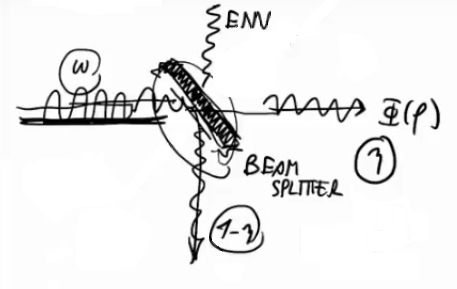
\includegraphics[width=0.7\linewidth]{BS}
		\caption{Beam splitter}
		\label{fig:bs}
	\end{figure}
	We focus our attention on one single frequency $\omega$. We send in a signal from the left onto the beam splitter (B.S.). A fraction $\eta$ (called \emph{transmission coefficient}) of the energy is transmitted; a fraction $1-\eta$ is reflected down. The environment plays an active role even if it is in the vacuum state $\ket{0}_E$. Indeed the action of the beam splitter can be described by some unitary s.t.
	\[ \Phi(\rho) = \Tr_E\left[U (\rho\otimes \ket{0}_E\bra{0}) U^\dagger \right] \]
	
	
	
\end{document}